% ============================================================================================
% BAB III ANALISIS MASALAH
% Pembagian subbab tidak rigid dan dapat bervariasi. Bab ini minimal berisi analisis kebutuhan
% fungsional dan nonfungsional, analisis berbagai alternatif solusi yang dapat ditawarkan, dan
% metode pemilihan solusi yang diusulkan.
% ============================================================================================
\cleardoublepage
\chapter{ANALISIS MASALAH}
\label{chap:analisis-masalah}

\section{Analisis Kondisi Saat Ini}
Penelitian oleh \textcite{wozniak2021deep} mengusulkan sebuah pendekatan hibrida yang dinamakan \textit{Correlation Learning Mechanism} (CLM). Model ini mengintegrasikan \textit{Convolutional Neural Network} (CNN) dengan \textit{Artificial Neural Network} (ANN) klasik dalam satu arsitektur terpadu untuk mendeteksi tumor otak dari citra \textit{CT Scan}.

\begin{figure}[h]
	\centering
	\captionsetup{justification=centering}
	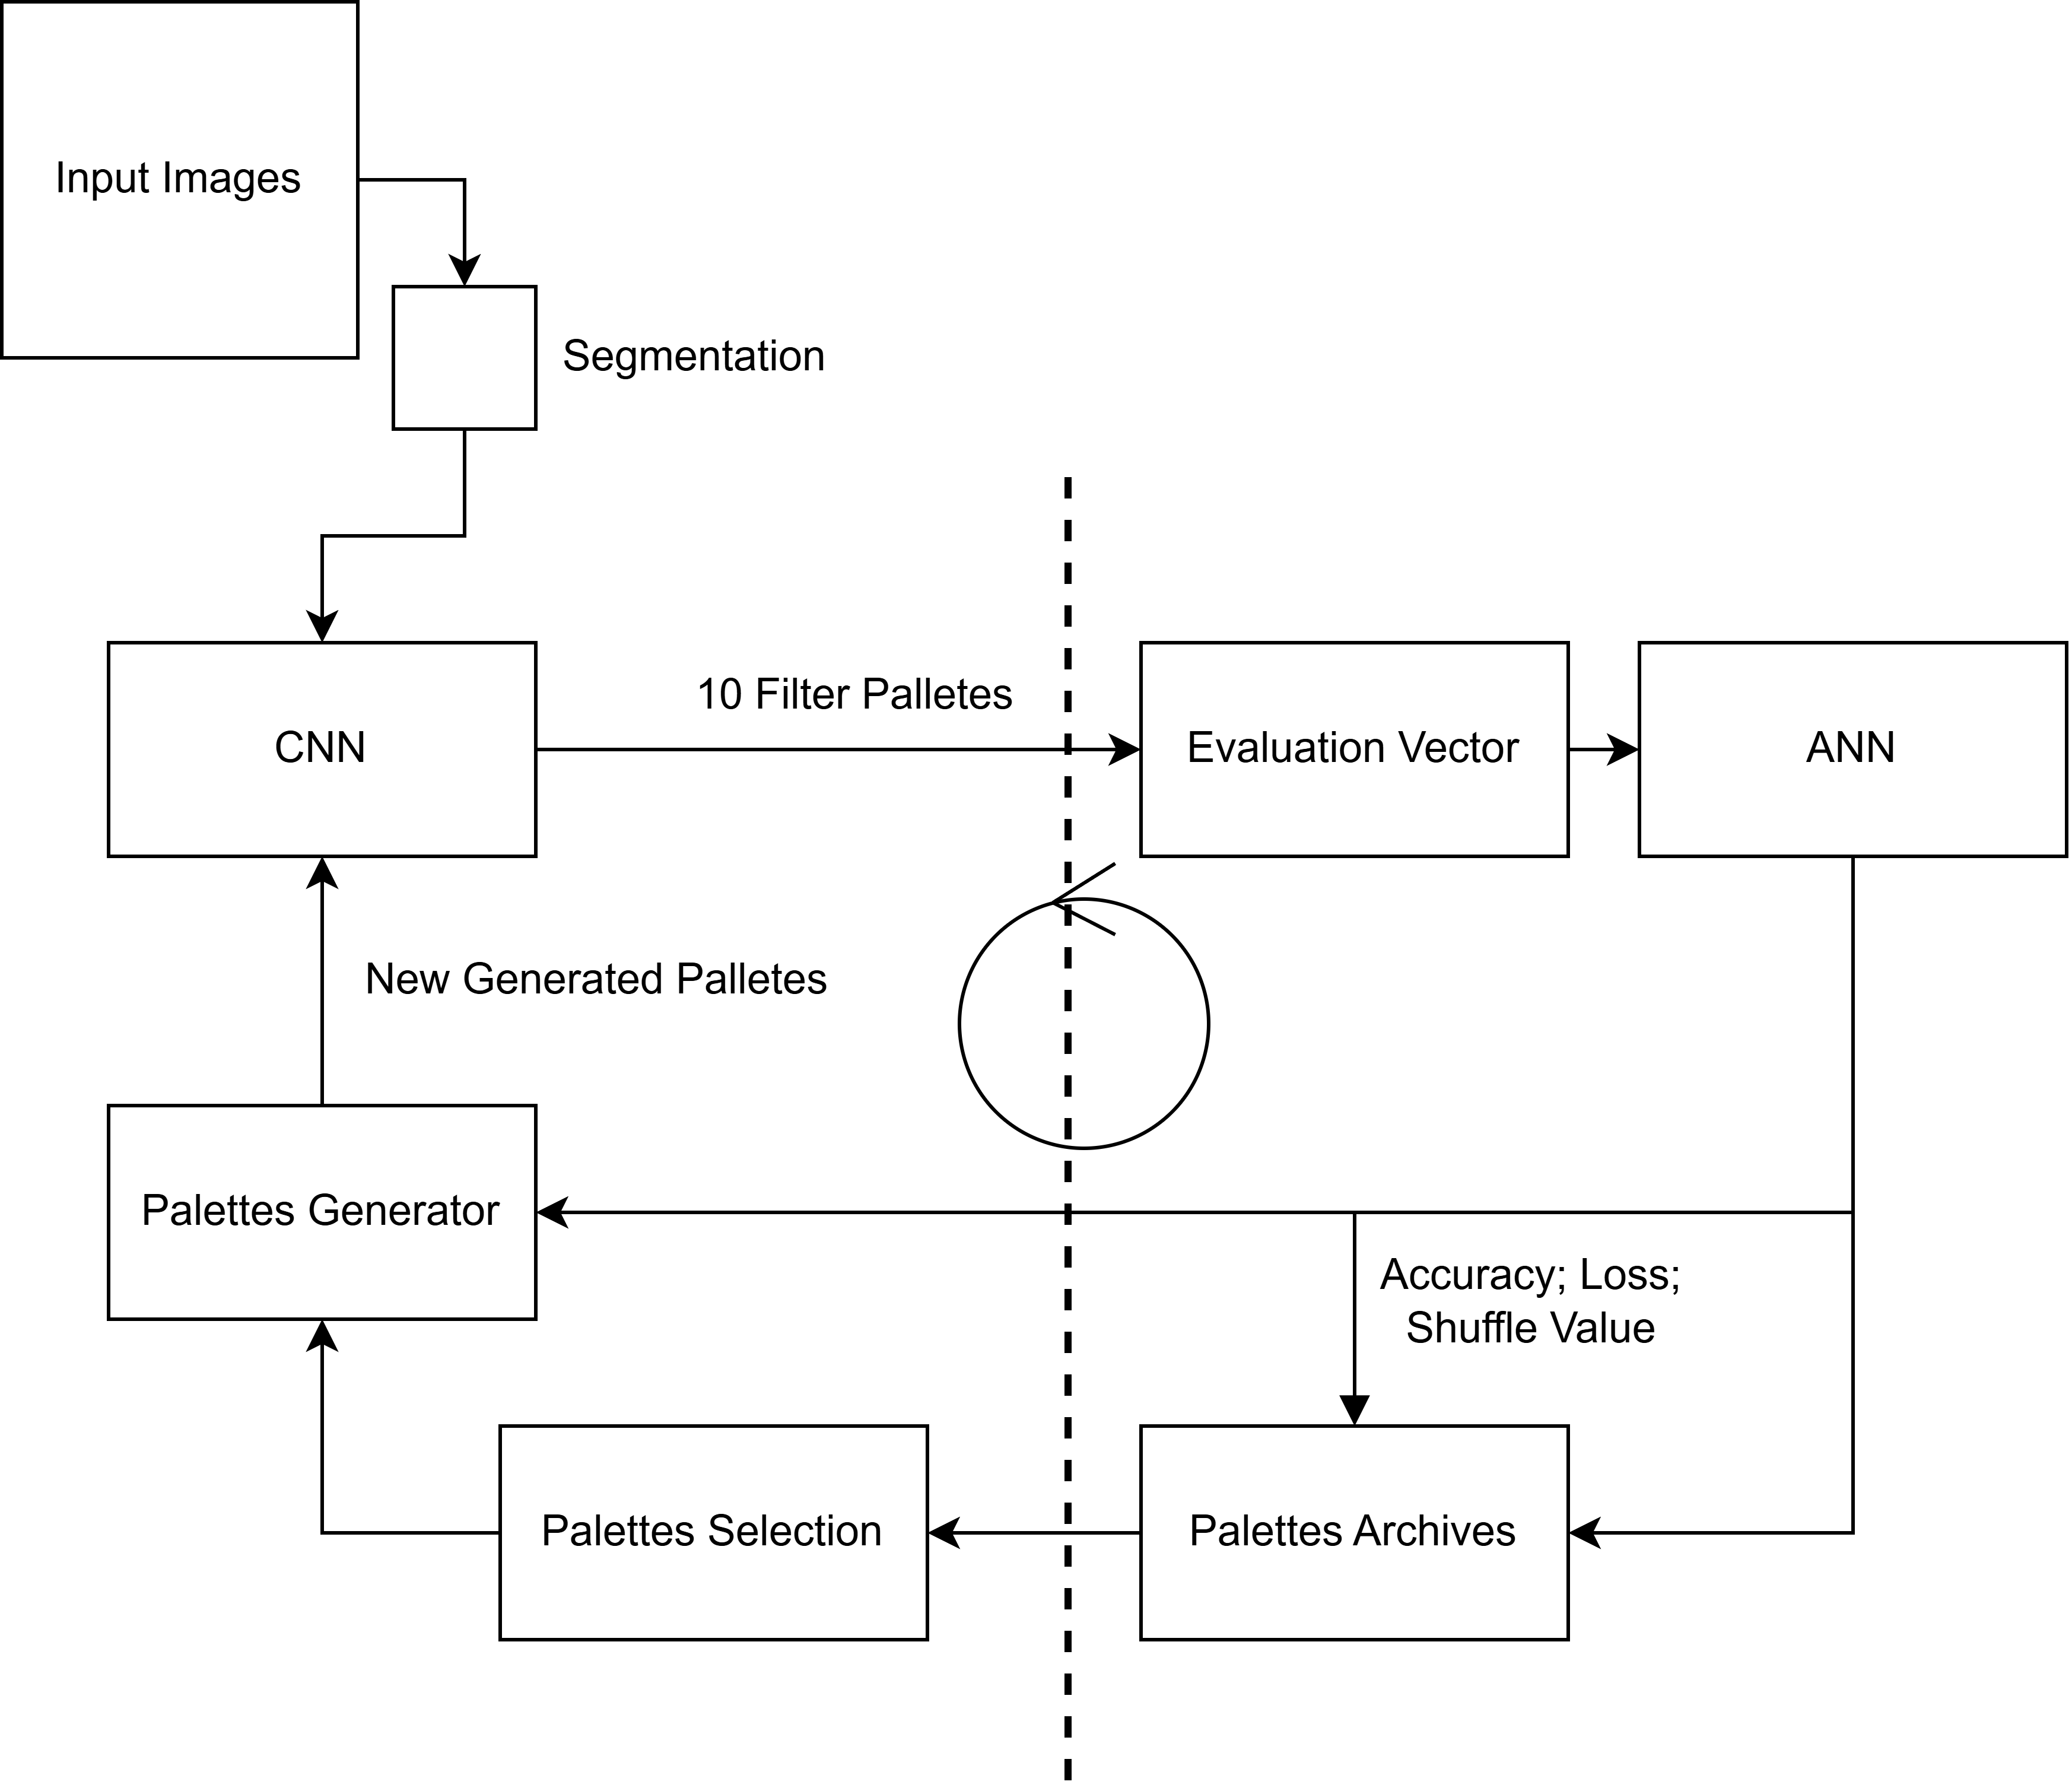
\includegraphics[width=0.7\textwidth]{images/Architecture.png}
	\caption{Visualisasi mekanisme \textit{Correlation Learning Mechanism} (CLM) \cite{wozniak2021deep}}
	\label{gambar:kondisisaatini}
\end{figure}

\subsection{Desain Sistem dan Mekanisme Kerja}
Sistem yang dikembangkan bekerja secara siklis dan iteratif dengan memanfaatkan pemrosesan paralel (\textit{multi-threading}). Berdasarkan Gambar \ref{gambar:kondisisaatini}, alur kerja sistem saat ini adalah sebagai berikut:
\begin{enumerate}
	\item Segmentasi \textit{Input}\\
	Citra \textit{CT Scan} otak dimasukkan ke dalam sistem dan disegmentasi menjadi 64 fragmen persegi. Jumlah fragmen ini dipilih secara spesifik untuk menyesuaikan dengan arsitektur CPU yang digunakan dalam penelitian tersebut guna menjaga keseimbangan antara kecepatan pembelajaran dan diversitas filter \cite{wozniak2021deep}.
	
	\item Mekanisme Palet Filter\\
	Fitur unik dari desain ini adalah penggunaan "palet filter" pada CNN. Palet ini merupakan konfigurasi dinamis yang menentukan lapisan, jenis filter, dan operasi (seperti \textit{pooling} dan ReLU). Pada iterasi awal, filter dipilih secara acak dari \textit{pool} filter yang tersedia, namun pada iterasi selanjutnya, pemilihan filter diatur oleh mekanisme CLM berdasarkan umpan balik akurasi \cite{wozniak2021deep}.
	
	\item Integrasi CNN-ANN\\
	CNN memproses fragmen gambar menggunakan palet yang terpilih. \textit{Output} dari CNN tidak hanya berupa \textit{feature maps}, tetapi juga dikonversi menjadi vektor deskripsi statistik numerik yang mencakup nilai minimum, maksimum, rata-rata aritmetika, jumlah, median, dan standar deviasi.
	
	\item Evaluasi dan Umpan Balik\\
	ANN bertindak sebagai evaluator. Data statistik dan fitur dari CNN menjadi \textit{input} bagi ANN untuk menghasilkan keputusan biner (tumor/sehat). Jika efisiensi ANN rendah, sistem melakukan pengacakan ulang (\textit{reshuffling}) pada palet filter CNN untuk iterasi berikutnya. Palet yang menghasilkan \textit{loss} terendah dan akurasi tertinggi disimpan dalam arsip basis data untuk digunakan kembali.
\end{enumerate}

\subsection{Peran Model}
Dalam arsitektur hibrida ini, masing-masing model memiliki peran spesifik yang saling bergantung:

\begin{enumerate}
	\item \textit{Convolutional Neural Network} (CNN)\\
	CNN berperan sebagai ekstraktor fitur yang adaptif. CNN tidak memiliki bobot filter yang statis seperti pada CNN konvensional, melainkan belajar untuk memilih kombinasi filter yang paling relevan untuk menonjolkan fitur tumor berdasarkan instruksi dari mekanisme korelasi. CNN juga bertugas menyederhanakan informasi visual kompleks menjadi deskripsi statistik yang lebih ringkas untuk diproses oleh ANN.
	\item \textit{Artificial Neural Network} (ANN)\\
	ANN berperan sebagai \textit{classifier} dan pengendali optimasi. ANN tidak hanya mengklasifikasikan keberadaan tumor, tetapi juga berfungsi sebagai mekanisme umpan balik bagi CNN. Performa ANN menjadi penentu apakah konfigurasi filter CNN saat ini harus dipertahankan atau diganti. Struktur ANN yang digunakan adalah \textit{fully connected layers} dengan arsitektur yang dipilih untuk melakukan kompresi data akhir.
\end{enumerate}

\subsection{Kelemahan dan Keterbatasan Sistem}
Model CLM yang diusulkan mampu mencapai akurasi tinggi hingga 96\% tetapi terdapat beberapa kelemahan dan keterbatasan yang menjadi celah pengembangan sebagai berikut \cite{wozniak2021deep}.

\begin{enumerate}
	\item Keterbatasan Kontrol Bobot Filter\\
	Dalam bagian \textit{future works}, peneliti mengakui bahwa sistem saat ini belum menerapkan pembobotan khusus (\textit{special weights}) pada filter di lapisan CNN. Hal ini membatasi kemampuan sistem untuk mengontrol proses penyaringan secara lebih halus agar \textit{feature maps} dapat menonjolkan objek kunci dengan lebih detail.
	\item Ketergantungan pada Iterasi Tetap\\
	Proses optimasi dan pelatihan dilakukan dalam jumlah iterasi yang tetap, seperti 120.000 iterasi atau seratus iterasi per \textit{batch} dalam algoritma \textit{multi threading}) sehingga prosesnya tidak dinamis seperti fungsi \textit{fitness}. Hal ini berpotensi menyebabkan inefisiensi waktu komputasi atau konvergensi yang belum optimal \cite{wozniak2021deep}.
	\item Kurangnya Aspek \textit{Explainability} (XAI)\\
	Pada sistem ini, hanya terdapat kotak merah yang tidak menandai otak secara keseluruhan yang memiliki tumor otak. Selain hal tersebut, sistem ini belum menerapkan metode \textit{Explainable AI} (XAI) yang mendalam untuk menjelaskan mengapa keputusan tersebut diambil. Interaksi antara statistik numerik dari CNN dan keputusan ANN masih bersifat \textit{black-box}, tanpa visualisasi kontribusi fitur yang mendetail, seperti \textit{heatmap} atau nilai SHAP untuk mendukung diagnosis klinis yang transparan. 
\end{enumerate}

\section{Analisis Kebutuhan}
Berdasarkan referensi studi literatur mengenai tinjauan komprehensif tentang tantangan dan arahan masa depan \textit{Artificial Intelligence} di layanan kesehatan oleh \textcite{ennab2024enhancing} dan tinjauan mengenai permasalahan \textit{black-box} berdasarkan prinsip etika ``\textit{do no harm}'' oleh \textcite{xu2023medical}, terdapat permasalahan yang ada di sistem \textit{deep learning} oleh \textcite{wozniak2021deep}, yaitu ketiadaan keterangan atau penjelasan mengenai \textit{black-box} dari \textit{deep learning} untuk mengetahui bagian mana yang terdeteksi tumor otak.

\subsection{Identifikasi Masalah Pengguna}
Terdapat dua kelompok pengguna utama yang menghadapi masalah terkait penerapan AI dalam medis, yaitu profesional medis (dokter dan radiolog) serta pasien.
Bagi profesional medis, tantangan utamanya tidak hanya terletak pada adopsi teknologi baru, tetapi juga pada keterbatasan manusiawi dan beban kerja yang ekstrem dalam praktik klinis. Berdasarkan \textcite{zhang2023diagnostic}, tingkat kesalahan diagnostik dalam radiologi berkisar antara 10-26\% dengan 60-80\% kesalahan  diklasifikasikan sebagai kesalahan perseptual atau kegagalan dalam mendeteksi adanya lesi. Faktor kelelahan turut berperan signifikan dengan survei mencatat 47\% radiolog mengalami \textit{burnout} dan 58\% mengalami gejala fisik seperti kelelahan mata yang dapat mengganggu akurasi interpretasi.

Di Indonesia, masalah ini menjadi jauh lebih kritis akibat ketimpangan rasio tenaga medis. Data analisis pasar layanan radiologi mencatat bahwa Indonesia hanya memiliki sekitar 2.161 radiolog terdaftar untuk melayani populasi sebesar 277 juta jiwa, atau setara dengan rasio 1,2 radiolog per 100.000 penduduk \autocite{insights102023indonesia}. Kondisi kekurangan SDM ini secara langsung meningkatkan beban kerja radiolog, yang berpotensi memperparah risiko \textit{burnout} dan kesalahan diagnosis. Selain itu,
profesional medis juga menghadapi masalah rendahnya kepercayaan terhadap keandalan sistem AI. Masalah ini berakar dari kurangnya edukasi, pelatihan, dan minimnya keterlibatan mereka dalam proses pengembangan sistem \autocite{syaftahan2025transformasi}. Hal ini menciptakan paradoks bahwa teknologi yang sangat dibutuhkan untuk mengurangi \textit{human error} justru diragukan validitasnya oleh penggunanya sendiri.

Dari sisi pasien, tantangan utama yang menghambat adopsi \textit{Artificial Intelligence} (AI) dalam praktik klinis adalah kurangnya kepercayaan terhadap validitas diagnosis yang melibatkan algoritma. Berbeda dengan asumsi umum bahwa teknologi canggih akan meningkatkan rasa aman pasien, literatur terbaru justru menunjukkan fenomena sebaliknya, yaitu keterlibatan AI sering kali dipersepsikan sebagai faktor yang mendegradasi kualitas layanan medis.
Riset eksperimental terbaru yang dilakukan oleh \textcite{chen2025impact} memberikan bukti bahwa kepercayaan pasien terhadap dokter dan intensi untuk melakukan pengobatan mencapai titik tertinggi justru ketika dokter secara eksplisit menyatakan tidak menggunakan AI dalam proses diagnosisnya dengan skor rata-rata kepercayaan 0,63. Sebaliknya, ketika pasien mengetahui bahwa dokter menggunakan AI secara ekstensif, tingkat kepercayaan mereka menurun ke angka 0,30 \autocite{chen2025impact}. Hal ini mengindikasikan bahwa di mata pasien, penggunaan AI belum dianggap sebagai peningkatan kapabilitas diagnostik, melainkan sebagai substitusi yang mengurangi nilai keahlian manusia.

Penurunan kepercayaan ini bukan tanpa alasan. Skeptisisme pasien berakar pada beberapa kekhawatiran fundamental. Pertama, risiko halusinasi AI, seperti model generatif dapat memproduksi informasi medis yang terdengar masuk akal dan meyakinkan tetapi secara faktual salah atau dibuat-buat. Ketakutan akan diagnosis yang keliru akibat kesalahan algoritma ini menjadi penghalang psikologis utama. Kedua, masalah transparansi dan akuntabilitas. Pasien sering kali memandang AI sebagai \textit{black-box} yang proses pengambilan keputusannya tidak dapat dijelaskan secara intuitif, memicu keraguan apakah keputusan medis tersebut didasarkan pada kondisi unik pasien atau sekadar pola statistik semata \autocite{chen2025impact}.
Selain itu, terdapat korelasi negatif antara persepsi profesionalisme dan penggunaan AI. Pasien cenderung mempertanyakan kompetensi dan penilaian klinis dokter yang terlalu bergantung pada alat bantu AI, terutama jika alat tersebut bersifat umum dan tidak dirancang khusus untuk medis. Penggunaan alat semacam ini dianggap mengaburkan batas tanggung jawab profesional dan menurunkan standar interaksi manusiawi yang menjadi inti dari layanan kesehatan \autocite{chen2025impact}. Temuan ini menegaskan bahwa diperlukan transparansi, validasi klinis yang ketat, dan jaminan pengawasan manusia untuk mengatasi ketidakpercayaan pasien.

Untuk mengatasi masalah tersebut, perlu didefinisikan kebutuhan fungsional dan nonfungsional sistem. Rincian kebutuhan ini akan dijabarkan pada subbab berikutnya.

\subsection{Kebutuhan Fungsional}
Berdasarkan analisis kebutuhan, kebutuhan fungsional sistem yang diinginkan adalah sebagai berikut.
\begin{enumerate}
	\item Sistem harus dapat menerima \textit{input} data berupa citra digital \textit{CT Scan} otak dengan format umum medis berupa DICOM.
	
	\item Sistem harus mampu melakukan segmentasi citra menjadi fragmen-fragmen untuk persiapan ekstraksi fitur.
	
	\item Sistem harus mampu mengklasifikasikan citra \textit{input} ke dalam dua kelas keputusan, yaitu tumor atau sehat.
	
	\item Sistem harus memiliki modul yang menampilkan matriks performa model yang telah tervalidasi untuk menilai performa kuantitatif dari sistem.
	
	\item Sistem harus menghasilkan visualisasi interpretasi keputusan model menggunakan metode \textit{Explainable AI} (XAI) untuk menyoroti area fitur pada citra yang dianggap indikatif terhadap tumor.
	
	\item Sistem harus menampilkan tingkat kepercayaan dari hasil prediksi untuk membantu tenaga medis dalam menilai validitas keputusan sistem dan membangun kepercayaan pengguna.
	
\end{enumerate}

\subsection{Kebutuhan Nonfungsional}
Kebutuhan nonfungsional sistem adalah sebagai berikut.

\begin{enumerate}
	\item \textit{Interpretability}\\
	Sistem harus mampu menyediakan transparansi atas keputusan yang diambil. Berbeda dengan sistem sebelumnya yang bersifat \textit{black-box}, sistem yang diusulkan harus memvisualisasikan area fokus, seperti penggunaan \textit{heatmap} yang menjadi dasar prediksi tumor. Hal ini bertujuan untuk menjawab keraguan pasien akan validitas diagnosis AI dan membantu profesional medis memverifikasi hasil tanpa harus mempercayai algoritma secara buta.
	
	\item \textit{Reliability}\\
	Sistem harus memiliki tingkat konsistensi yang tinggi dalam memberikan hasil prediksi. Mengingat risiko kesalahan diagnostik radiologi berkisar antara 10-26\%, sistem diharapkan dapat mempertahankan atau melampaui akurasi model referensi (96\%).
	
	\item \textit{Efficiency}\\
	Waktu komputasi untuk memproses satu citra \textit{input} hingga menghasilkan diagnosis dan visualisasi harus memiliki waktu yang singkat agar tidak menghambat alur kerja klinis.
\end{enumerate}

\section{Analisis Pemilihan Solusi}
Pada bagian ini, dilakukan analisis kebutuhan untuk menentukan solusi yang paling tepat dalam mengatasi permasalahan \textit{black-box} pada model AI. Tahapan analisis ini mencakup identifikasi dan pemaparan berbagai alternatif solusi dan menggunakan metodologi AHP untuk mengevaluasi dan memilih solusi terbaik dari alternatif tersebut.

\subsection{Alternatif Solusi}
Alternatif solusi yang dapat diberikan dalam permasalahan tersebut terbagi menjadi dua, yaitu penggunaan metode XAI pada infrastruktur yang sama dan penggunaan model yang berbeda untuk mencegah terjadinya \textit{black-box} pada AI.

Alternatif solusi pertama fokus pada penerapan metode XAI yang dapat menyelesaikan masalah \textit{black-box}, khususnya dalam konteks \textit{computer vision} (\textit{CT scan}) dan model CNN yang sudah ada. Penjelasan mendalam mengenai metode-metode berikut dapat dilihat pada Bab \ref{sec:metode_xai}, Subbab \nameref{sec:metode_xai}.

\begin{enumerate}
	\item \textit{Attribution-based methods} \\
	\textit{Attribution-based methods} memberi nilai pada setiap bagian masukan gambar. Bagian yang paling memengaruhi keputusan akhir akan mendapat nilai tinggi. Hal ini dapat membantu penggunanya untuk melihat area mana pada gambar yang paling penting bagi AI. Alternatif solusi yang menggunakan \textit{attribution-based methods} adalah sebagai berikut.
	\begin{enumerate}
		\item \textit{Gradient-weighted Class Activation Mapping} (Grad-CAM)
		
		\item FullGrad-CAM dan FullGrad-CAM++
		
		\item \textit{SmoothGrad}
	\end{enumerate}
	
	\item \textit{Transformer-based methods}
	\textit{Transformer-based methods} memanfaatkan mekanisme \textit{attention} bawaan pada arsitektur \textit{Vision Transformer} (ViT). Teknik ini membagi gambar menjadi beberapa \textit{patch} dan memvisualisasikan skor atensinya menjadi peta yang menyoroti area paling krusial dalam pengambilan keputusan model \autocite{iftikhar2025explainable}.
\end{enumerate}

Selain mengevaluasi berbagai metode XAI untuk disematkan pada arsitektur \textit{deep learning} yang ada, analisis ini juga memperhitungkan alternatif penggunaan model yang berbeda secara mendasar, seperti model \textit{machine learning} konvensional. Perbandingan komprehensif antara pendekatan \textit{deep learning} berbasis XAI dengan model konvensional (baik yang bersifat \textit{white-box} maupun \textit{black-box}) diperlukan untuk membuktikan efektivitas dan urgensi dari solusi yang diusulkan dalam tugas akhir ini.

Analisis penentuan solusi yang digunakan pada tugas akhir ini menggunakan \textit{Analytic Hierarchy Process} (AHP). AHP adalah metode pengambilan keputusan yang digunakan oleh individu atau organisasi untuk melakukan pemeringkatan alternatif yang mereka pertimbangkan berdasarkan perbandingan berpasangan. \textit{Analytic Hierarchy Process} (AHP) melibatkan lima langkah utama. Pertama, menyusun hierarki masalah keputusan ke dalam tiga tingkatan, yaitu tujuan, kriteria, dan alternatif. Kedua, melakukan perbandingan berpasangan untuk kriteria guna menilai kepentingan relatifnya menggunakan skala sembilan poin, mulai dari rasio 1 yang berarti sama penting hingga rasio 9 yang berarti sangat penting, serta nilai kebalikannya. Ketiga, menghitung bobot kriteria untuk mewakili kepentingan relatifnya, yang diturunkan dari rasio preferensi pada langkah sebelumnya. Keempat, mengevaluasi alternatif dengan melakukan perbandingan berpasangan serupa untuk setiap pasangan alternatif berdasarkan setiap kriteria. Kelima, menggabungkan bobot kriteria dan skor alternatif melalui perkalian dan penjumlahan untuk menghasilkan skor total bagi setiap alternatif, yang kemudian digunakan untuk memeringkatnya \autocite{1000minds2025ahp}.

AHP pada tugas akhir dilakukan berdasarkan literatur yang melakukan evaluasi terhadap model terkait. Terdapat tiga studi literatur yang digunakan untuk menganalisis alternatif solusi, yaitu:

\begin{enumerate}
	\item \textit{Explainable AI and vision transformers for detection and classification of brain tumor: a comprehensive survey} \cite{hosny2025explainable} \\
	Penelitian ini membahas tentang tinjauan teknis dan perbandingan teknik diagnostik \textit{deep learning} (DL) untuk tumor otak, dengan fokus pada penelitian dari tahun 2020 hingga 2024, seperti CNN, \textit{transfer learning}, \textit{vision transformers} (ViT), teknik hibrida, dan \textit{Explainable AI} (XAI). Tugas akhir ini mengeksplorasi kinerja, keunggulan, dan keterbatasan dari pendekatan-pendekatan tersebut pada \textit{dataset} umum seperti Figshare dan BraTS.
	
	\item \textit{Explainable CNN for brain tumor detection and classification through XAI based key features identification} \cite{iftikhar2025explainable}\\
	Penelitian ini menggunakan metodologi yang menggabungkan \textit{Explainable AI} (XAI) dengan arsitektur CNN untuk mengatasi masalah model yang kompleks dan sulit diinterpretasi. Tugas akhir ini menggunakan teknik XAI berupa \textit{Gradient-weighted Class Activation Mapping} (Grad-CAM) agar memastikan model fokus pada fitur tumor yang relevan.
	
	\item \textit{Optimizing brain tumor classification through feature selection and hyperparameter tuning in machine learning models} \autocite{tahosin2023optimizing}\\
	Penelitian ini memberikan data perbandingan algoritma \textit{machine learning}. Hasilnya menunjukkan bahwa \textit{Extra Trees} mencapai akurasi tertinggi (98\%) dan \textit{Naive Bayes} memiliki akurasi terendah (69\%) namun sangat efisien secara komputasi.
\end{enumerate}

Tahapan AHP yang dilakukan adalah sebagai berikut:
\begin{enumerate}
	\item Struktur Hierarki Keputusan
	\begin{enumerate}
		\item Tujuan \\
		Memilih pendekatan \textit{deep learning} atau \textit{machine learning} yang paling efektif dan sesuai untuk tugas klasifikasi atau deteksi penyakit dari data medis.
		\item Kriteria
		\begin{enumerate}
			\item C1: Akurasi Deteksi \\
			Kemampuan model untuk secara benar mengidentifikasi atau mengklasifikasikan kondisi medis.
			\item C2: \textit{Interpretability} \\
			Kemampuan model untuk memberikan penjelasan atas prediksinya, yang krusial dalam konteks medis untuk membangun kepercayaan dan memahami fokus model.
			\item C3: \textit{Robustness} dan Generalisasi \\
			Kemampuan model untuk berkinerja baik pada data baru (\textit{unseen data}) atau \textit{dataset} yang berbeda, serta ketahanan terhadap variasi data.
			\item C4: Kebutuhan Data dan Teknik \textit{Preprocessing}\\
			Sensitivitas model terhadap jumlah data yang tersedia dan efektivitas teknik seperti augmentasi data, \textit{transfer learning}, atau \textit{preprocessing} spesifik.
			\item C5: Kompleksitas Model \\
			Ukuran arsitektur, seperti jumlah \textit{layer}, parameter yang dapat memengaruhi interpretasi, efisiensi, dan risiko \textit{overfitting}.
		\end{enumerate}
		\item Alternatif Solusi
		\begin{enumerate}
			\item A1: CNN + Grad-CAM (Mewakili \textit{attribution-based methods})
			\item A2: \textit{Vision Transformer }(ViT) + \textit{Attention Map }(Mewakili Transformer-based methods)
			\item A3: \textit{Naive Bayes} (Representasi \textit{white-box})
			\item A4: \textit{Extra Trees} (Representasi \textit{black-box})
		\end{enumerate}
	\end{enumerate}
	\item Perbandingan Berpasangan Antar Kriteria \\
	Perbandingan berpasangan dilakukan berdasarkan kriteria yang ada untuk menentukan prioritas dari setiap kriteria. Perbandingan antarkriteria dilakukan menggunakan matriks perbandingan berpasangan kriteria. Matriks perbandingan berpasangan kriteria adalah tabel yang merekam hasil perbandingan preferensi antara setiap pasang kriteria, menggunakan skala sembilan poin untuk menunjukkan tingkat kepentingan satu kriteria terhadap yang lain. Hasil dari matriks perbandingan kriteria dapat dilihat pada Tabel \ref{tab:perbandingan_kriteria}.
	\begin{table}[H]
		\centering
		\caption{Matriks Perbandingan Berpasangan Kriteria}
		\label{tab:perbandingan_kriteria}
		\begin{tabular}{|l|c|c|c|c|c|}
			\hline
			Kriteria & C1 & C2 & C3 & C4 & C5 \\ \hline
			C1 (Akurasi) & $1$ & $1$ & $5$ & $3$ & $5$ \\ \hline
			C2 (XAI) & $1$ & $1$ & $5$ & $3$ & $5$ \\ \hline
			C3 (Efisiensi) & $1/5$ & $1/5$ & $1$ & $1/3$ & $1$ \\ \hline
			C4 (Data) & $1/3$ & $1/3$ & $3$ & $1$ & $3$ \\ \hline
			C5 (Kompleksitas) & $1/5$ & $1/5$ & $1$ & $1/3$ & $1$ \\ \hline
		\end{tabular}
	\end{table}
	Setelah dilakukan perbandingan, dilakukan normalisasi ke vektor prioritas kriteria. Normalisasi dilakukan dengan cara matriks perbandingan dikuadratkan, kemudian setiap baris dijumlahkan, dan hasil penjumlahan setiap baris dibagi dengan total keseluruhan jumlah baris. Langkah-langkah tersebut diulangi pada matriks hasil hingga nilai vektor prioritas yang dihasilkan menjadi konvergen \textcite{1000minds2025ahp}. Hasil dari vektor prioritas kriteria dapat dilihat pada Tabel \ref{tab:prioritas_kriteria}.
	\begin{table}[h]
		\centering
		\caption{Vektor Prioritas Kriteria}
		\label{tab:prioritas_kriteria}
		\begin{tabular}{|l|r|r|}
			\hline
			Kriteria & Bobot & Prioritas (\%) \\ \hline
			C1: Akurasi & 359 & 35,9\% \\ \hline
			C2: \textit{Interpretability} & 359 & 35,9\% \\ \hline
			C3: \textit{Robustness}/Generalisasi & 64 & 6,4\% \\ \hline
			C4: Kebutuhan Data & 153 & 15,3\% \\ \hline
			C5: Kompleksitas Model & 64 & 6,4\% \\ \hline
			Total & 1.000 & 100,0\% \\ \hline
		\end{tabular}
	\end{table}
	\item Perbandingan Berpasangan Antar Alternatif \\
	Perbandingan dilakukan dengan cara setiap alternatif dibandingkan dengan alternatif solusi lain berdasarkan masing-masing kriteria menggunakan matriks perbandingan berpasangan kriteria \textcite{1000minds2025ahp}. Setelah itu, dilakukan normalisasi yang sama dengan perhitungan prioritas kriteria. Perbandingan antaralternatif berdasarkan kriteria dan prioritas alternatif solusi dapat dilihat pada Tabel \ref{tab:perbandingan_c1} hingga Tabel \ref{tab:perbandingan_c5}.
	\begin{table}[H]
		\centering
		\caption{Matriks Perbandingan Berpasangan C1 (Akurasi)}
		\label{tab:perbandingan_c1}
		\begin{tabular}{|l|c|c|c|c|}
			\hline
			C1: Akurasi & A1 & A2 & A3 & A4 \\ \hline
			A1 & $1$ & $2$ & $7$ & $4$ \\ \hline
			A2 & $1/2$ & $1$ & $5$ & $3$ \\ \hline
			A3 & $1/7$ & $1/5$ & $1$ & $1/3$ \\ \hline
			A4 & $1/4$ & $1/3$ & $3$ & $1$ \\ \hline
		\end{tabular}
	\end{table}
	
	Berdasarkan Tabel \ref{tab:perbandingan_c1}, dihasilkan pembobotan dengan menggunakan normalisasi sebagai berikut:
	\begin{enumerate}
		\item A1: 50,5\%
		\item A2: 30,6\%
		\item A3: 5,8\%
		\item A4: 13,1\%\\
	\end{enumerate}
	
	Pendekatan CNN dengan Grad-CAM (A1) memperoleh bobot tertinggi karena arsitektur CNN, terutama yang menggunakan \textit{transfer learning}, secara konsisten mendominasi performa akurasi dalam analisis citra medis dan terbukti lebih stabil pada \textit{dataset} standar. \textit{Vision Transformer} (A2) masih menghadapi tantangan generalisasi jika data latih terbatas, sedangkan \textit{Naive Bayes} (A3) memiliki performa paling rendah dengan akurasi sekitar 69\% yang dinilai kurang memadai untuk diagnosis kritis.
	
	\begin{table}[H]
		\centering
		\caption{Matriks Perbandingan Berpasangan C2 (Interpretability)}
		\label{tab:perbandingan_c2}
		\begin{tabular}{|l|c|c|c|c|}
			\hline
			C2: XAI & A1 & A2 & A3 & A4 \\ \hline
			A1 & $1$ & $3$ & $2$ & $7$ \\ \hline
			A2 & $1/3$ & $1$ & $1/3$ & $3$ \\ \hline
			A3 & $1/2$ & $3$ & $1$ & $7$ \\ \hline
			A4 & $1/7$ & $1/3$ & $1/7$ & $1$ \\ \hline
		\end{tabular}
	\end{table}
	
	Berdasarkan Tabel \ref{tab:perbandingan_c2}, dihasilkan pembobotan dengan menggunakan normalisasi sebagai berikut:
	\begin{enumerate}
		\item A1: 47,4\%
		\item A2: 13,9\%
		\item A3: 33,4\%
		\item A4: 5,3\%\\
	\end{enumerate}
	
	Metode CNN yang dilengkapi Grad-CAM (A1) unggul karena mampu menghasilkan visualisasi \textit{heatmap} yang menyoroti area tumor berdasarkan gradien lapisan konvolusi terakhir sehingga memberikan transparansi keputusan yang sangat dibutuhkan. \textit{Naive Bayes} (A3) menempati posisi kedua karena sifatnya sebagai model \textit{white-box} yang mudah dijelaskan secara matematis, berbeda dengan \textit{Extra Trees} (A4) yang merupakan model \textit{ensemble} (\textit{black-box}) yang sulit dilacak alur keputusannya. Sementara itu, peta atensi pada ViT (A2) sering kali menangkap hubungan global yang lebih abstrak dibandingkan fitur fisik tumor sehingga interpretasi visualnya lebih sulit dipahami dibandingkan \textit{heatmap} CNN.
	
	\begin{table}[H]
		\centering
		\caption{Matriks Perbandingan Berpasangan C3 (Efisiensi Komputasi)}
		\label{tab:perbandingan_c3}
		\begin{tabular}{|l|c|c|c|c|}
			\hline
			C3: Efisiensi & A1 & A2 & A3 & A4 \\ \hline
			A1 & $1$ & $3$ & $1/7$ & $1/3$ \\ \hline
			A2 & $1/3$ & $1$ & $1/9$ & $1/5$ \\ \hline
			A3 & $7$ & $9$ & $1$ & $3$ \\ \hline
			A4 & $3$ & $5$ & $1/3$ & $1$ \\ \hline
		\end{tabular}
	\end{table}
	
	Berdasarkan Tabel \ref{tab:perbandingan_c3}, dihasilkan pembobotan dengan menggunakan normalisasi sebagai berikut:
	\begin{enumerate}
		\item A1: 10,1\%
		\item A2: 4,9\%
		\item A3: 60,7\%
		\item A4: 24,3\%\\
	\end{enumerate}
	
	\textit{Naive Bayes} (A3) mendominasi kriteria ini karena kesederhanaan algoritmanya yang membutuhkan sumber daya komputasi minimal dan waktu pelatihan yang cepat. \textit{Extra Trees} (A4) juga dinilai efisien karena struktur \textit{tree}-nya yang mengurangi redundansi data. Metode berbasis \textit{deep learning} seperti CNN (A1) dan \textit{Vision Transformer} (A2) memiliki beban komputasi yang jauh lebih berat, seperti ViT yang memproses gambar sebagai urutan \textit{patch} dengan mekanisme atensi yang memakan memori besar dan waktu pelatihan yang jauh lebih lama dibandingkan metode konvensional.
	
	\begin{table}[H]
		\centering
		\caption{Matriks Perbandingan Berpasangan C4 (Kebutuhan Data)}
		\label{tab:perbandingan_c4}
		\begin{tabular}{|l|c|c|c|c|}
			\hline
			C4: Data & A1 & A2 & A3 & A4 \\ \hline
			A1 & $1$ & $3$ & $1/5$ & $1/3$ \\ \hline
			A2 & $1/3$ & $1$ & $1/7$ & $1/5$ \\ \hline
			A3 & $5$ & $7$ & $1$ & $2$ \\ \hline
			A4 & $3$ & $5$ & $1/2$ & $1$ \\ \hline
		\end{tabular}
	\end{table}
	
	Berdasarkan Tabel \ref{tab:perbandingan_c4}, dihasilkan pembobotan dengan menggunakan normalisasi sebagai berikut:
	\begin{enumerate}
		\item A1: 12,2\%
		\item A2: 5,7\%
		\item A3: 52,3\%
		\item A4: 29,8\%\\
	\end{enumerate}
	
	Alternatif \textit{Naive Bayes} (A3) dan \textit{Extra Trees} (A4) lebih unggul karena kemampuan mereka untuk bekerja efektif dan tidak mudah \textit{overfitting} pada \textit{dataset} dengan jumlah sampel yang sedikit. Sebaliknya, CNN (A1) membutuhkan jumlah data yang besar atau strategi augmentasi data untuk mencapai generalisasi yang baik, dan \textit{Vision Transformer} (A2) mendapatkan bobot terendah karena arsitekturnya tidak memiliki bias induktif sehingga memerlukan \textit{dataset} berskala besar agar performanya tidak menurun drastis.
	
	\begin{table}[H]
		\centering
		\caption{Matriks Perbandingan Berpasangan C5 (Kompleksitas)}
		\label{tab:perbandingan_c5}
		\begin{tabular}{|l|c|c|c|c|}
			\hline
			C5: Kompleksitas & A1 & A2 & A3 & A4 \\ \hline
			A1 & $1$ & $2$ & $1/7$ & $1/3$ \\ \hline
			A2 & $1/2$ & $1$ & $1/8$ & $1/4$ \\ \hline
			A3 & $1/7$ & $8$ & $1$ & $3$ \\ \hline
			A4 & $3$ & $4$ & $1/3$ & $1$ \\ \hline
		\end{tabular}
	\end{table}
	
	Berdasarkan Tabel \ref{tab:perbandingan_c5}, dihasilkan pembobotan dengan menggunakan normalisasi sebagai berikut:
	\begin{enumerate}
		\item A1: 9,4\%
		\item A2: 6,0\%
		\item A3: 60,8\%
		\item A4: 23,8\%\\	
	\end{enumerate}
	
	Dalam aspek kompleksitas arsitektur, \textit{Naive Bayes} (A3) dinilai paling sederhana karena hanya mengandalkan perhitungan probabilitas statistik dasar, diikuti oleh \textit{Extra Trees} (A4). Sementara itu, CNN (A1) memiliki struktur hierarkis yang dalam dengan jutaan parameter yang harus dilatih, dan \textit{Vision Transformer} (A2) dinilai paling kompleks karena mekanisme \textit{multi-head self-attention} yang memiliki kompleksitas kuadratik terhadap jumlah token (\textit{patch} gambar), menjadikannya model yang paling berat secara struktural dibandingkan alternatif lainnya.
	
	\item Perbandingan Berpasangan Setiap Pasangan Alternatif Berdasarkan Setiap Kriteria \\
	Setelah perbandingan dilakukan pada setiap alternatif berdasarkan kriteria, dilakukan penggabungan perbandingan pada setiap pasangan alternatif berdasarkan setiap kriteria dengan hasil yang dapat dilihat pada Tabel \ref{tab:hasil_perhitungan}.
	\begin{table}[h]
		\centering
		\caption{Hasil Perhitungan Perbandingan Berpasangan}
		\label{tab:hasil_perhitungan}
		\begin{tabular}{|l|c|c|c|c|c|c|}
			\hline
			Alternatif & C1 & C2 & C3 & C4 & C5 & Hasil Akhir \\ \hline
			Bobot Kriteria & 35,9\% & 35,9\% & 6,4\% & 15,3\% & 6,4\% & \\ \hline
			A1 & 505 & 474 & 101 & 122 & 94 & 382,607 \\ \hline
			A2 & 306 & 139 & 49 & 57 & 60 & 175,452 \\ \hline
			A3 & 58 & 334 & 607 & 523 & 608 & 298,507 \\ \hline
			A4 & 131 & 53 & 243 & 298 & 238 & 142,434 \\ \hline
		\end{tabular}
	\end{table}
	Perhitungan Rinci Skor Akhir:
	\begin{enumerate}
		\item A1 (CNN + Grad-CAM): $(0,359 \times 505) + (0,359 \times 474) + (0,064 \times 101) + (0,153 \times 122) + (0,064 \times 94) = 382,607$
		\item A2 (ViT + Attention Map): $(0,359 \times 306) + (0,359 \times 139) + (0,064 \times 49) + (0,153 \times 57) + (0,064 \times 60) = 175,452$
		\item A3 (Naive Bayes): $(0,359 \times 58) + (0,359 \times 334) + (0,064 \times 607) + (0,153 \times 523) + (0,064 \times 608) = 298,507$
		\item A4 (Extra Trees): $(0,359 \times 131) + (0,359 \times 53) + (0,064 \times 243) + (0,153 \times 298) + (0,064 \times 238) = 142,434$
	\end{enumerate}
	\item Pemilihan Solusi \\
	Dengan mempertimbangkan bobot prioritas dan skor kinerja keseluruhan, model \textit{deep learning} yang menggunakan Grad-CAM (A1) ditetapkan sebagai solusi pada tugas akhir. Metode ini memberikan keseimbangan terbaik antara akurasi tinggi dan interpretabilitas kuat, sejalan dengan tujuan metodologi yang menekankan pada keandalan model sekaligus transparansi keputusan AI.
\end{enumerate}